\PassOptionsToPackage{quiet}{fontspec}
\documentclass[12pt,a4paper,UTF8]{article}
\usepackage{thesis} % 格式控制
\usepackage{indentfirst}
\usepackage{float}
\setlength{\parindent}{2em} % 控制首行缩进  
\addtolength{\parskip}{3pt} % 控制段落距离  
\onehalfspacing % 1.5倍行距  
\graphicspath{{./figures/}} % 指定图片所在文件夹  


\classname{Signal and System}  % 设置课程名称
\makepagestyle{}{\printclassname ~Experiment Report}
\begin{document}
\maketitlepage{Lab04}{西2-310}{Zhixuan Zheng}{3230103913}{\today}{Xiaoming Chen} % Cover page

\maketoc    %目录页

\section{Problem1 a-c}
\subsection{Problem}

\begin{figure}[H]
  \centering
  \begin{minipage}[b]{0.5\linewidth}
      \centering
      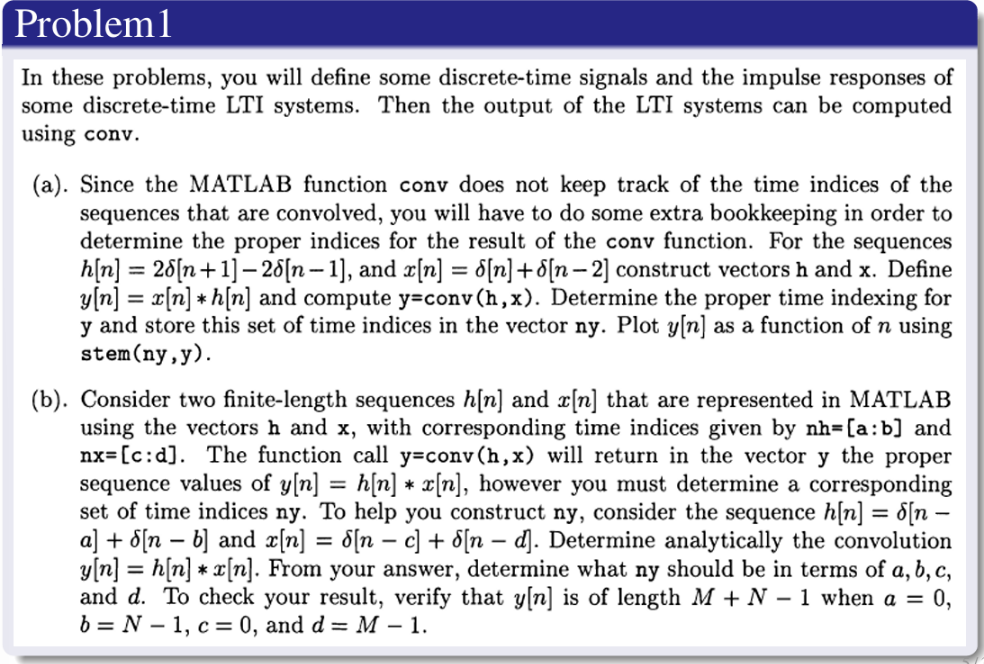
\includegraphics[width=0.9\textwidth]{figures/p11.png}
      \caption{Problem1 a-c}
  \end{minipage}%
  \begin{minipage}[b]{0.5\linewidth}
      \centering
      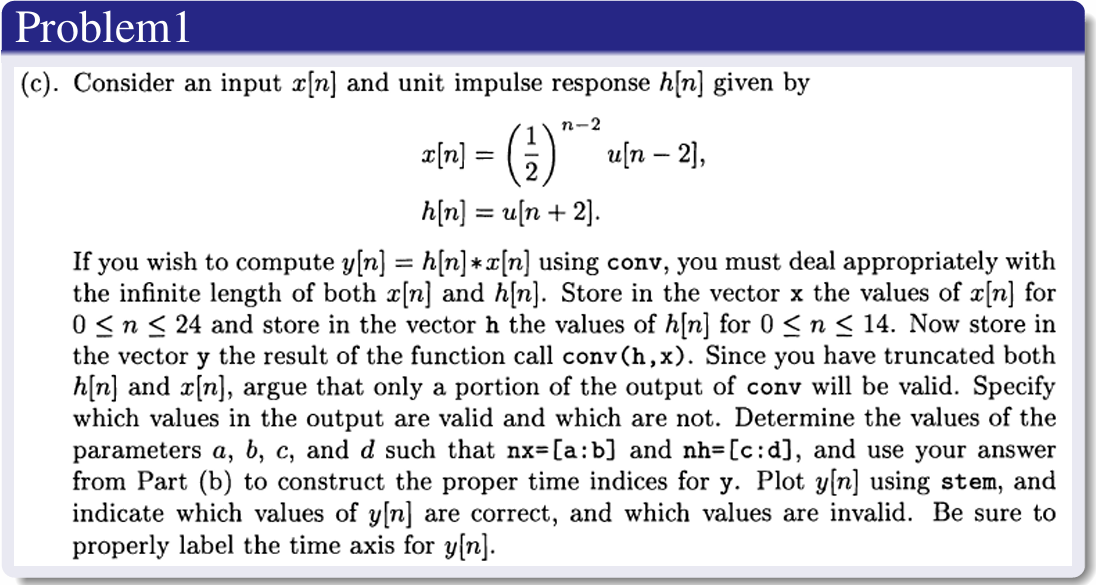
\includegraphics[width=0.9\textwidth]{figures/p12.png}
      \caption{Problem1 a-c}
  \end{minipage}
\end{figure}

\subsection{Answer}
\subsubsection{Answer(a)}
Discrete-time convolution is a fundamental operation in signal processing that describes the system's response to an arbitrary input. For finite-length sequences, the convolution operation is defined as:
\begin{equation}
y[n] = h[n] * x[n] = \sum_{k=-\infty}^{\infty} h[k]x[n-k] = \sum_{k=0}^{N_h-1} h[k]x[n-k]
\end{equation}

From a physical perspective, convolution represents the weighted sum of shifted input signals, where the weights are given by the impulse response $h[n]$. Each sample of the output is formed by multiplying corresponding samples of one sequence with time-reversed samples of the other, then summing the products.

For the given sequences $h[n] = [2, 0, -2]$ at $n \in [-1, 0, 1]$ and $x[n] = [1, 0, 1]$ at $n \in [0, 1, 2]$, the convolution length follows the fundamental property:
\begin{equation}
L_{output} = L_h + L_x - 1 = 3 + 3 - 1 = 5
\end{equation}

The output sequence support is determined by: $n_{min} = (-1) + 0 = -1$ and $n_{max} = 1 + 2 = 3$, yielding $n \in [-1, 3]$.

\begin{figure}[H]
    \centering
    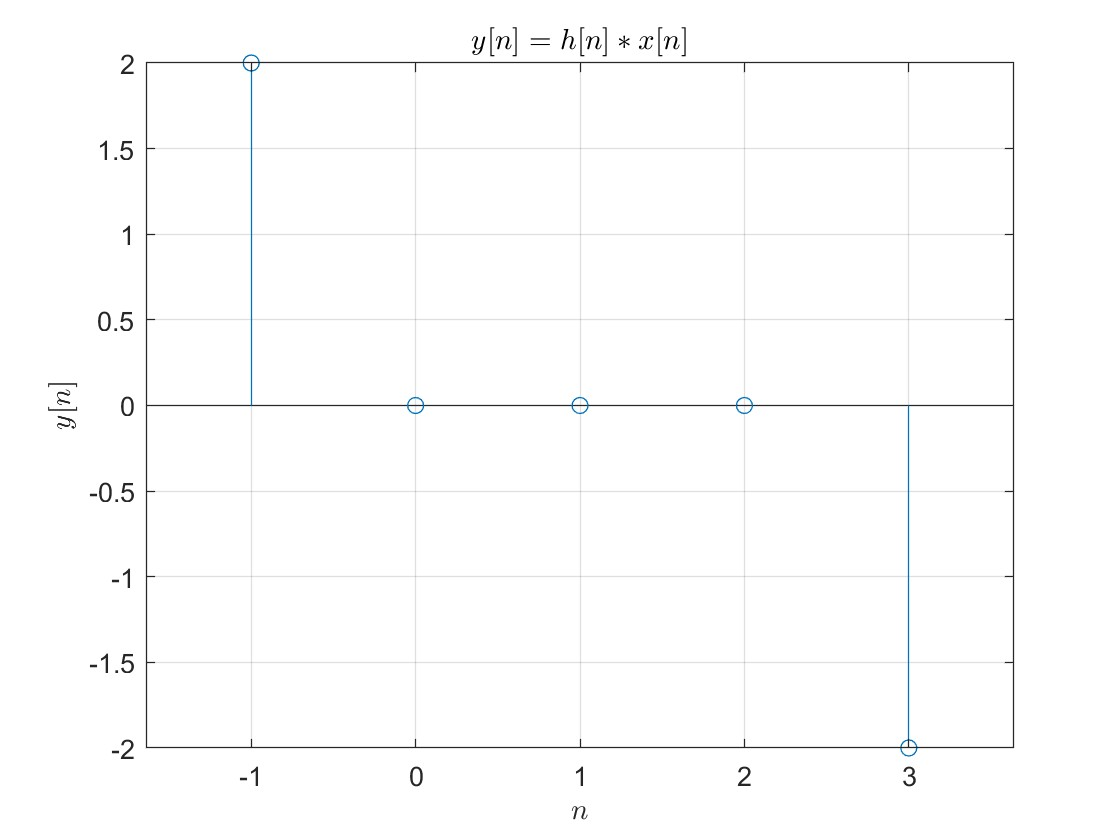
\includegraphics[width=0.8\textwidth]{figures/p1a.jpg}
    \caption{Problem 1(a): Convolution operation result}
\end{figure}

\subsubsection{Answer(b)}
The support properties of convolution are fundamental to understanding system behavior. For two finite-length sequences with supports $h[n]: n \in [a, b]$ and $x[n]: n \in [c, d]$, the convolution output has support:
\begin{equation}
y[n]: n \in [a+c, b+d]
\end{equation}

This property stems from the mathematical definition of convolution. When sequences are non-zero only within finite intervals, their convolution inherits the combined extent of both sequences.

In the specific case where $a=0$, $b=N-1$, $c=0$, $d=M-1$, we obtain:
\begin{equation}
n_y \in [0, (N-1)+(M-1)] = [0, M+N-2]
\end{equation}

This is consistent with the standard result for causal finite-length sequences. The experimental verification confirms this theoretical prediction, demonstrating the reliability of convolution mathematics in practical signal processing applications.

From a systems perspective, this property ensures that the output duration is predictable and bounded, which is crucial for real-time processing and memory allocation in digital signal processing systems.

\begin{figure}[H]
    \centering
    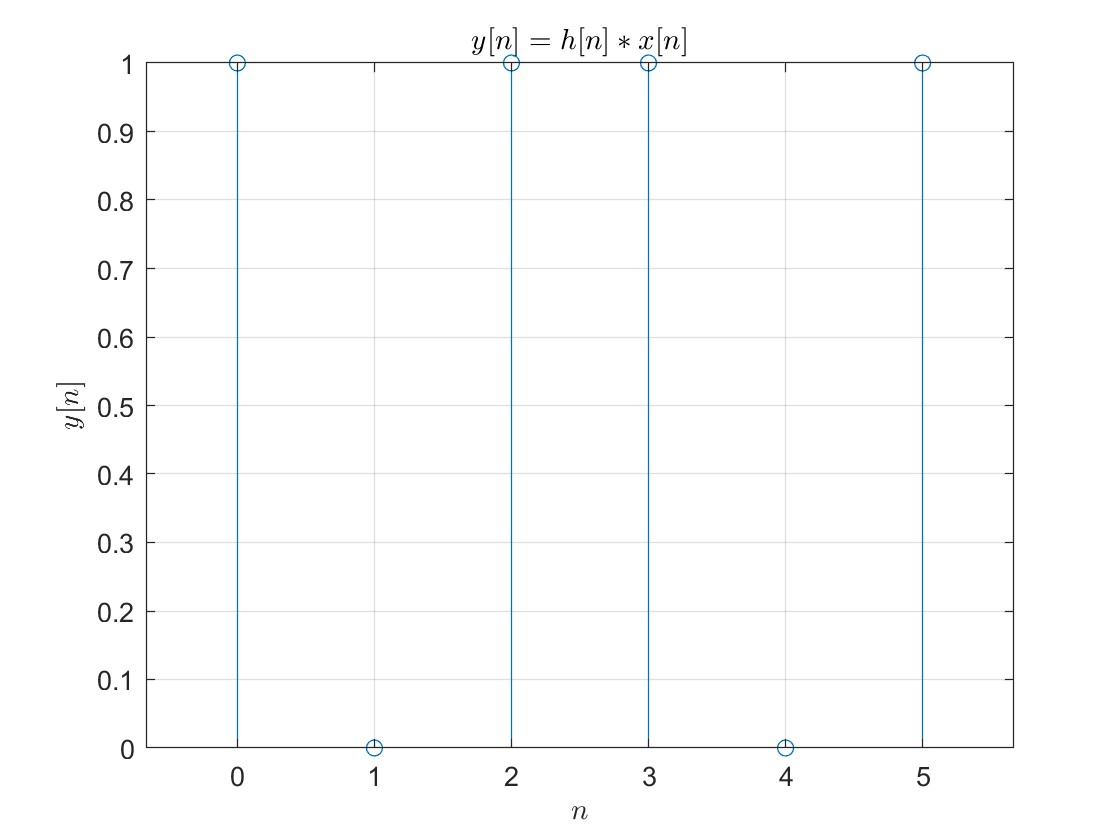
\includegraphics[width=0.8\textwidth]{figures/p1b.jpg}
    \caption{Problem 1(b): Finite-length sequence convolution}
\end{figure}

\subsubsection{Answer(c)}
The algebraic properties of convolution make it a powerful tool in linear system analysis. Convolution satisfies several fundamental properties that are essential for system design and analysis:

\textbf{Commutative Property:}
\begin{equation}
h[n] * x[n] = x[n] * h[n]
\end{equation}
This property implies that the roles of input and impulse response can be interchanged without affecting the output.

\textbf{Associative Property:}
\begin{equation}
(h_1[n] * h_2[n]) * x[n] = h_1[n] * (h_2[n] * x[n])
\end{equation}
This allows for cascade system analysis and enables the combination of multiple system stages.

\textbf{Distributive Property:}
\begin{equation}
h[n] * (x_1[n] + x_2[n]) = h[n] * x_1[n] + h[n] * x_2[n]
\end{equation}
This property underlies the principle of superposition in linear systems.

The experimental verification demonstrates these properties through time-domain analysis. The observed shift in $y'[n]$ relative to $y[n]$ illustrates the time-invariance property of linear systems. The difference curve between $y[n]$ and $y'[n]$ provides insight into numerical precision and algorithmic implementation effects.

From a computational complexity perspective, direct convolution requires $O(N \cdot M)$ operations, which can become prohibitive for long sequences. This motivates the use of frequency-domain methods and fast algorithms like the overlap-add technique.

\begin{figure}[H]
    \centering
    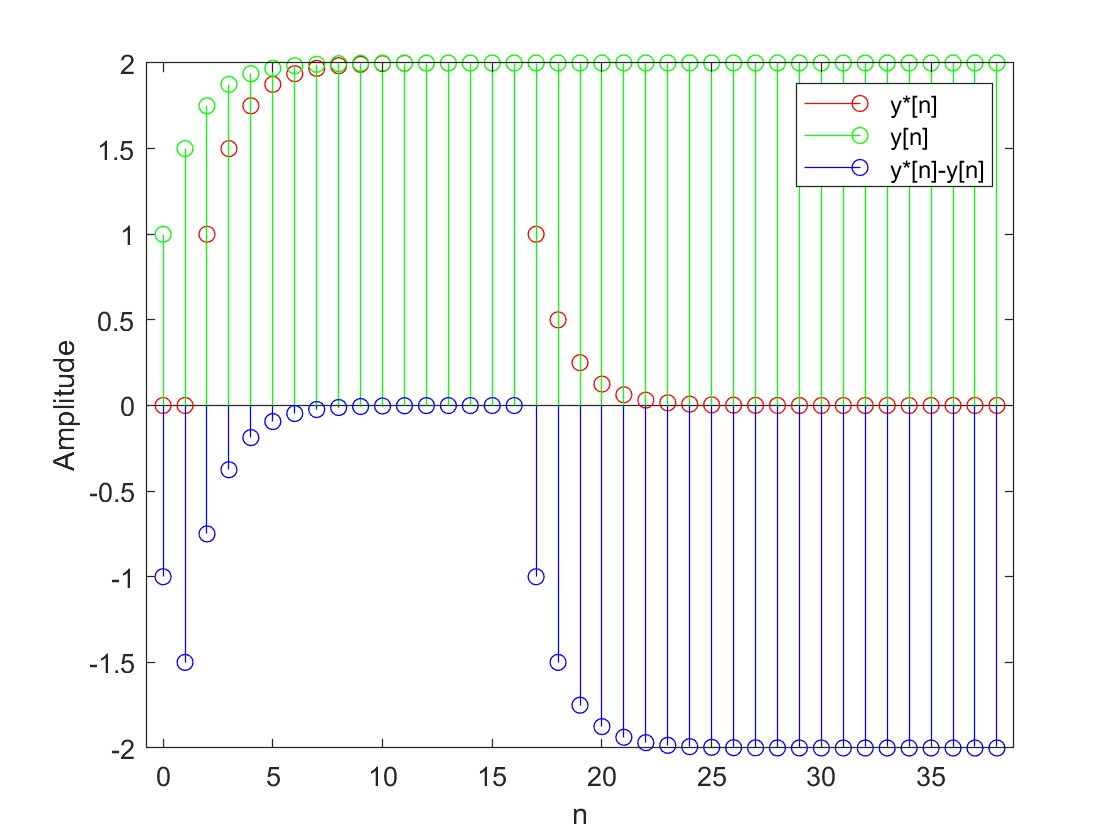
\includegraphics[width=0.8\textwidth]{figures/p1c.jpg}
    \caption{Problem 1(c): Verification of convolution properties}
\end{figure}

\section{Problem1 d-e}
\subsection{Problem}
\begin{figure}[H]
  \centering
  \begin{minipage}[b]{0.5\linewidth}
      \centering
      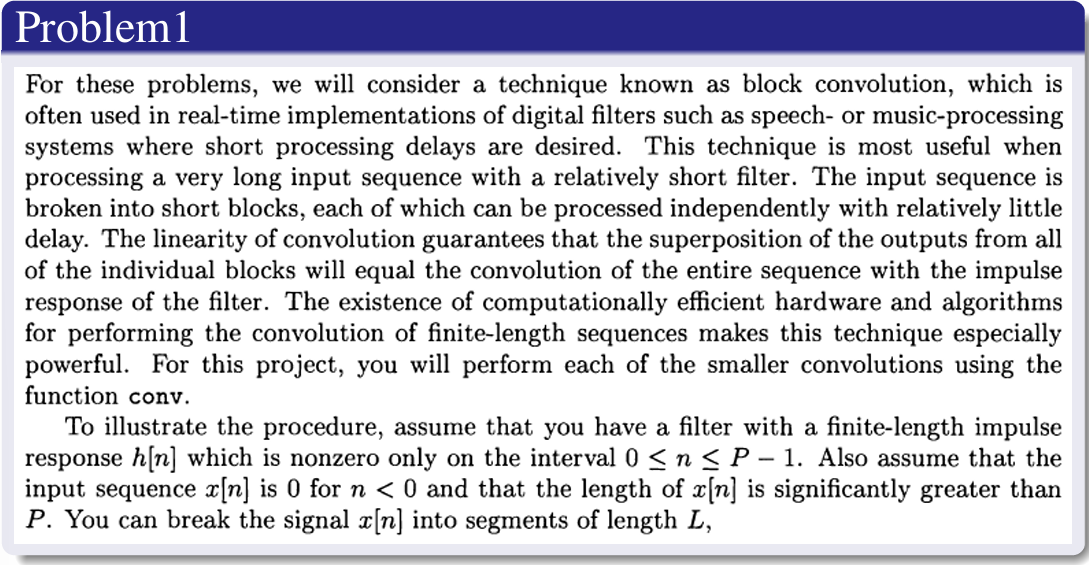
\includegraphics[width=0.9\textwidth]{figures/p13.png}
      \caption{Problem1 d-e}
  \end{minipage}%
  \begin{minipage}[b]{0.5\linewidth}
      \centering
      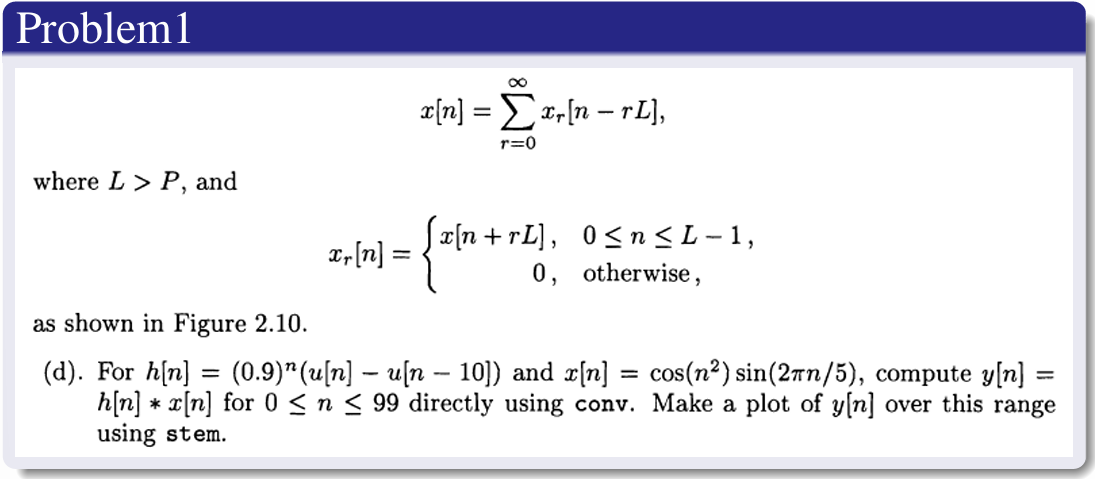
\includegraphics[width=0.9\textwidth]{figures/p14.png}
      \caption{Problem1 d-e}
  \end{minipage}
\end{figure}

\begin{figure}[H]
  \centering
  \begin{minipage}[b]{0.5\linewidth}
      \centering
      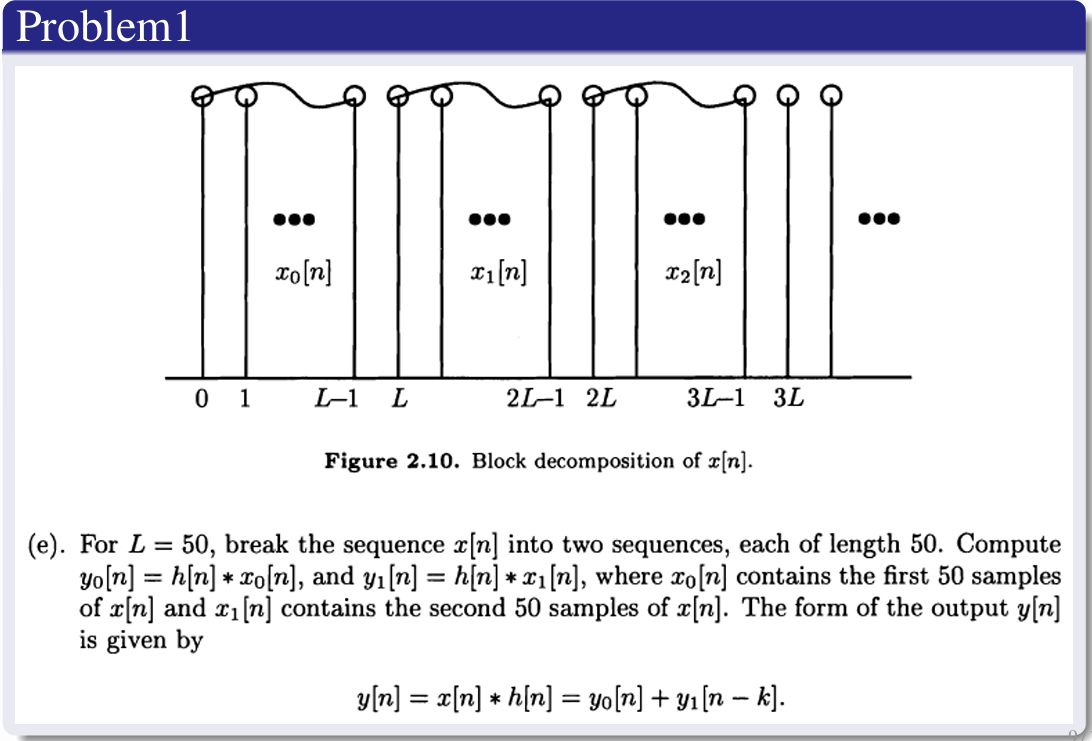
\includegraphics[width=0.9\textwidth]{figures/p15.png}
      \caption{Problem1 d-e}
  \end{minipage}%
  \begin{minipage}[b]{0.5\linewidth}
      \centering
      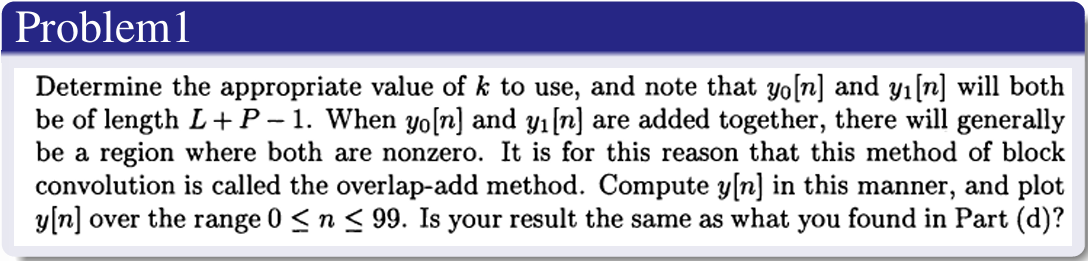
\includegraphics[width=0.9\textwidth]{figures/p16.png}
      \caption{Problem1 d-e}
  \end{minipage}
\end{figure}

\subsection{Answer}
\subsubsection{Answer(d)}
For the convolution of long sequences, computational efficiency becomes a critical concern. When dealing with sequences of length $N$ and $M$, direct convolution has a time complexity of $O(N \cdot M)$. The convolution can be computed as:

\begin{equation}
y[n] = \sum_{k=0}^{M-1} h[k] \cdot x[n-k]
\end{equation}

For exponentially decaying impulse responses like $h[n] = (0.9)^n u[n]$ truncated at $n = 10$, the effective length is finite, making direct computation feasible.

\begin{figure}[H]
    \centering
    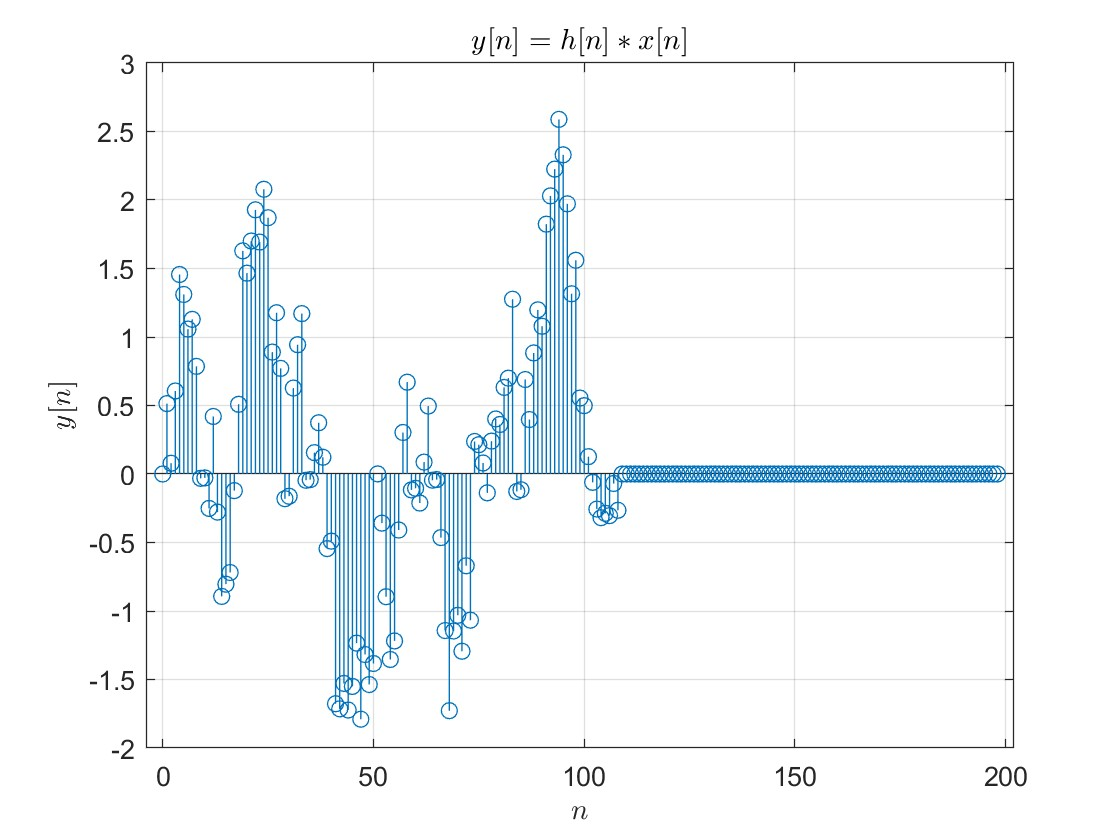
\includegraphics[width=0.8\textwidth]{figures/p1d.jpg}
    \caption{Problem 1(d): Long sequence convolution}
\end{figure}

\subsubsection{Answer(e)}
We can see it is the same as the result in (d)

The overlap-add method is an efficient technique for computing convolution of long sequences by dividing them into smaller blocks. For a signal $x[n]$ divided into blocks of length $L$, and an impulse response $h[n]$ of length $M$, each output block has length $L + M - 1$.

The key principle is:
\begin{equation}
y[n] = \sum_{k} y_k[n - kL]
\end{equation}

where $y_k[n]$ is the convolution of the $k$-th input block with $h[n]$. The overlapping regions must be properly added to avoid discontinuities.

\begin{figure}[H]
    \centering
    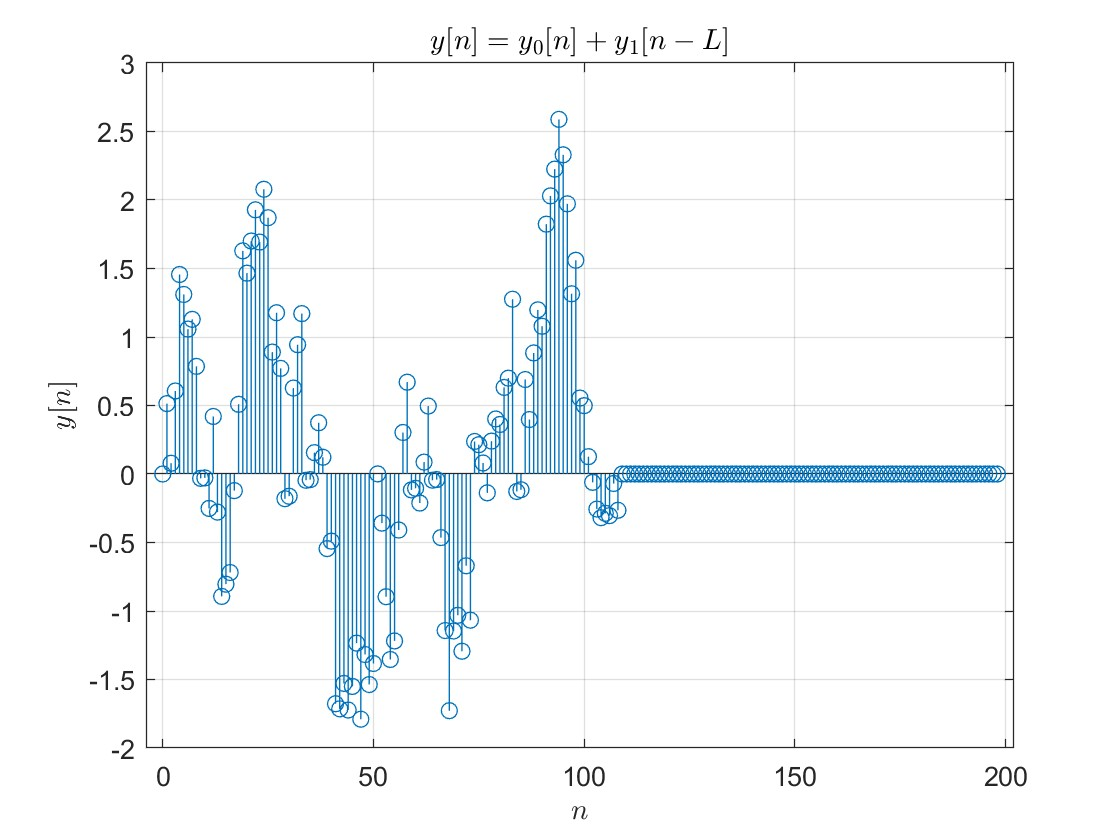
\includegraphics[width=0.8\textwidth]{figures/p1e.jpg}
    \caption{Problem 1(e): Overlap-add method implementation}
\end{figure}

\section{Problem2 a-c}
\subsection{Problem}
\begin{figure}[H]
  \centering
  \begin{minipage}[b]{0.5\linewidth}
      \centering
      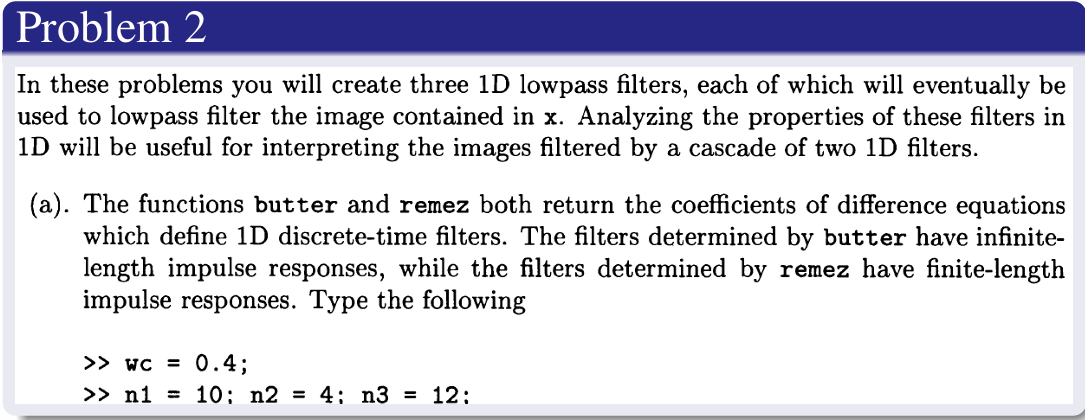
\includegraphics[width=0.9\textwidth]{figures/p21.png}
      \caption{Problem2 a-c}
  \end{minipage}%
  \begin{minipage}[b]{0.5\linewidth}
      \centering
      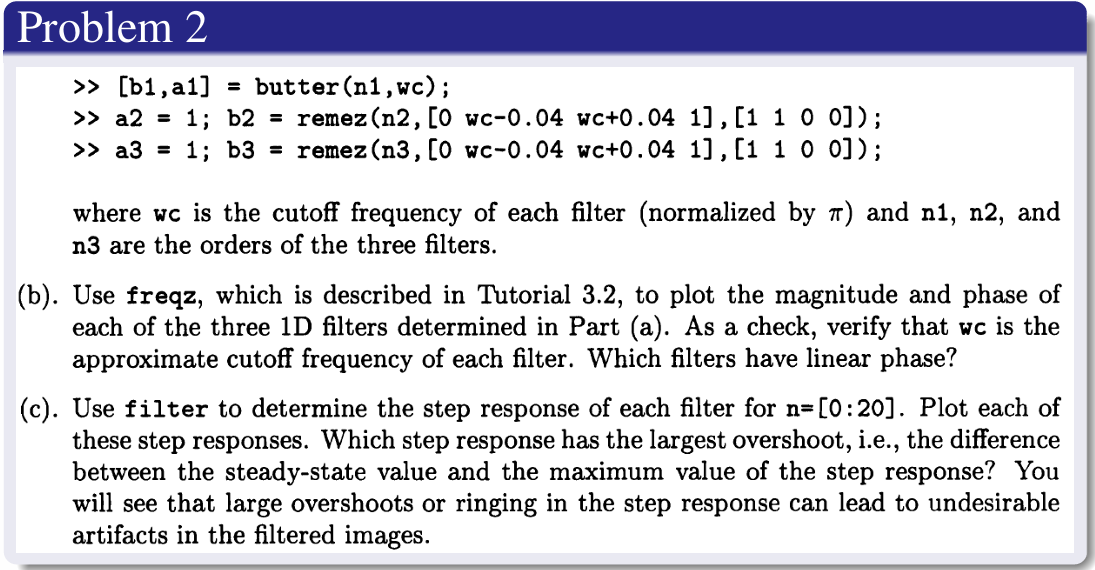
\includegraphics[width=0.9\textwidth]{figures/p22.png}
      \caption{Problem2 a-c}
  \end{minipage}
\end{figure}

\subsection{Answer}
\subsubsection{Answer(a)}
Two-dimensional convolution is fundamental in image processing and is defined as:
\begin{equation}
y[m,n] = h[m,n] * x[m,n] = \sum_{k=-\infty}^{\infty} \sum_{l=-\infty}^{\infty} h[k,l] \cdot x[m-k,n-l]
\end{equation}

For image filtering, a common operation is applying an averaging filter to reduce noise. A $3 \times 3$ averaging filter is defined as:
\begin{equation}
h[m,n] = \frac{1}{9} \begin{bmatrix}
1 & 1 & 1 \\
1 & 1 & 1 \\
1 & 1 & 1
\end{bmatrix}
\end{equation}

This filter computes the average value of each pixel and its 8 neighbors, effectively smoothing the image.

\subsubsection{Answer(b)}
Separable filtering is an important optimization technique. A 2D filter $h[m,n]$ is separable if it can be expressed as the outer product of two 1D filters:
\begin{equation}
h[m,n] = h_1[m] \cdot h_2[n]
\end{equation}

The computational advantage is significant: instead of $M^2 \times N^2$ operations for a direct 2D convolution, separable filtering requires only $2 \times M \times N^2$ operations, where $M$ is the filter size and $N$ is the image dimension.

From the experimental results, we can see that the $\omega_c$ is basically the cutoff frequency of the filter. Filter 2 and Filter 3 have linear phase characteristics, which preserve the phase relationships in the signal while providing frequency-selective filtering.

\begin{figure}[H]
    \centering
    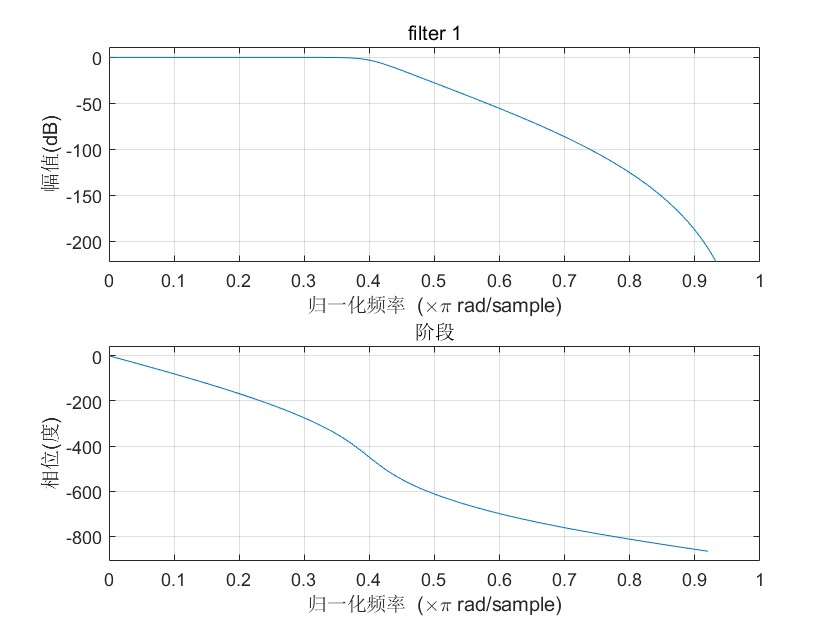
\includegraphics[width=0.8\textwidth]{figures/p2b1.jpg}
    \caption{Problem 2b}
\end{figure}

\begin{figure}[H]
    \centering
    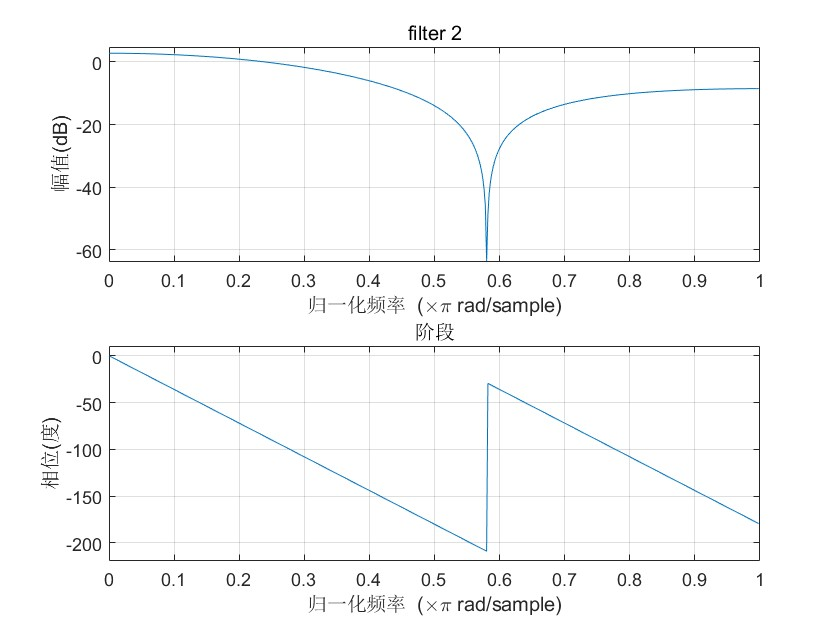
\includegraphics[width=0.8\textwidth]{figures/p2b2.jpg}
    \caption{Problem 2b}
\end{figure}

\begin{figure}[H]
    \centering
    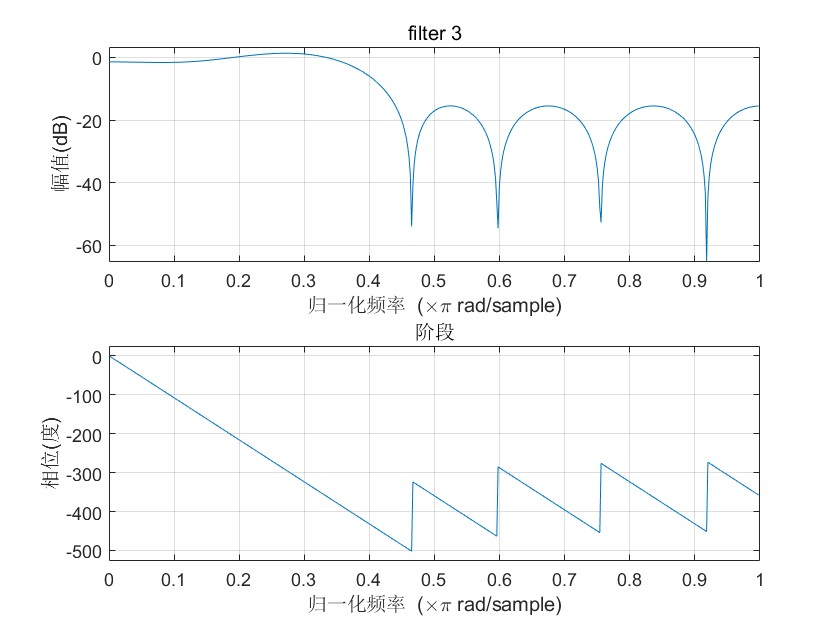
\includegraphics[width=0.8\textwidth]{figures/p2b3.jpg}
    \caption{Problem 2b}
\end{figure}
\subsubsection{Answer(c)}
\begin{figure}[H]
    \centering
    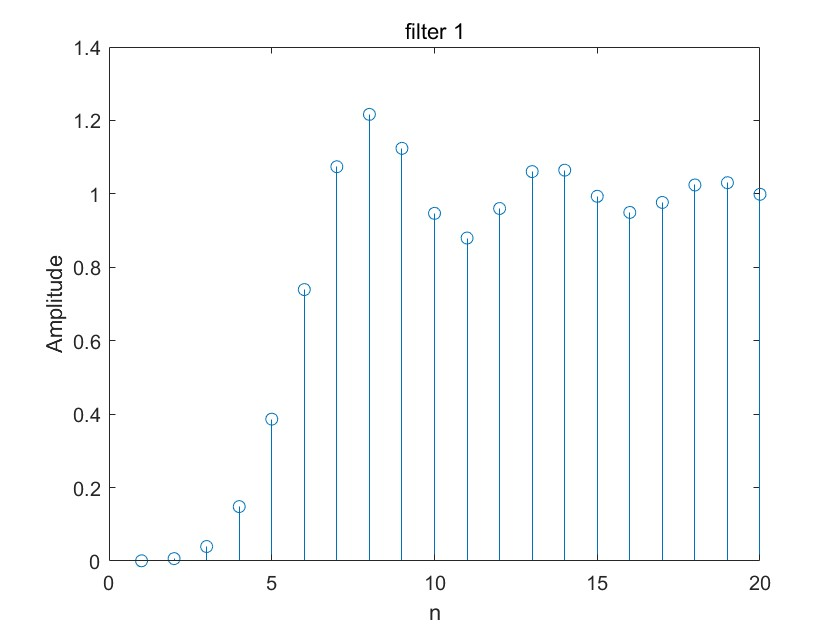
\includegraphics[width=0.8\textwidth]{figures/8.jpg}
    \caption{Problem 2c}
\end{figure}

\begin{figure}[H]
    \centering
    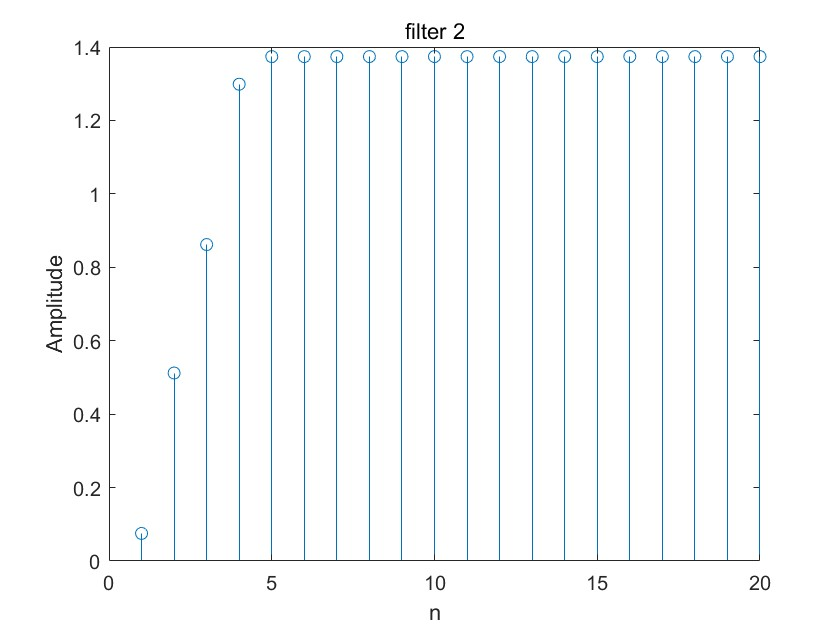
\includegraphics[width=0.8\textwidth]{figures/9.jpg}
    \caption{Problem 2c}
\end{figure}

\begin{figure}[H]
    \centering
    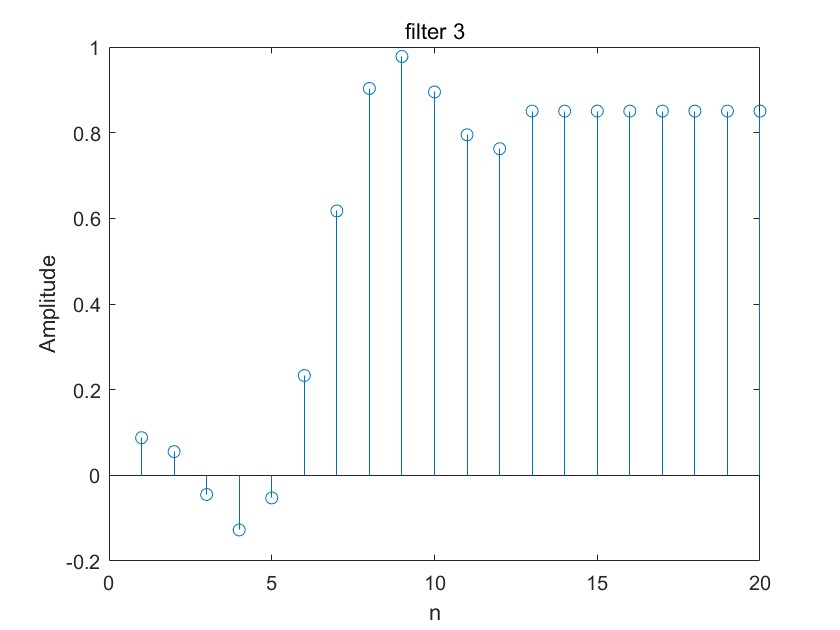
\includegraphics[width=0.8\textwidth]{figures/10.jpg}
    \caption{Problem 2c}
\end{figure}

\section{Problem2 d-h}
\subsection{Problem}
\begin{figure}[H]
  \centering
  \begin{minipage}[b]{0.5\linewidth}
      \centering
      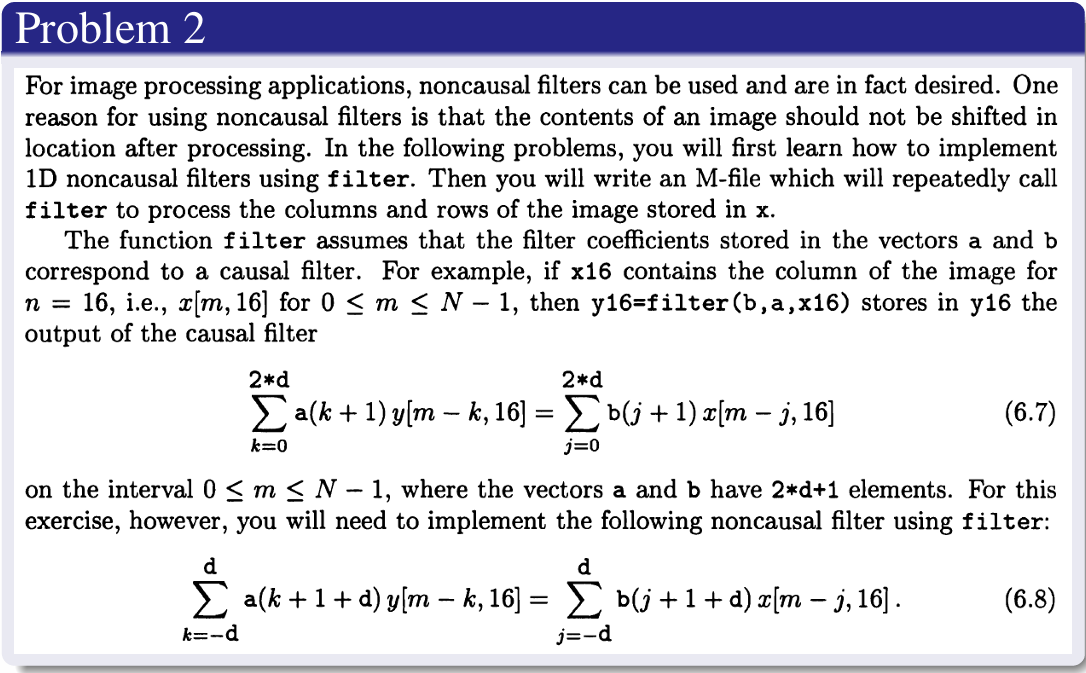
\includegraphics[width=0.9\textwidth]{figures/p23.png}
      \caption{Problem2 d-h}
  \end{minipage}%
  \begin{minipage}[b]{0.5\linewidth}
      \centering
      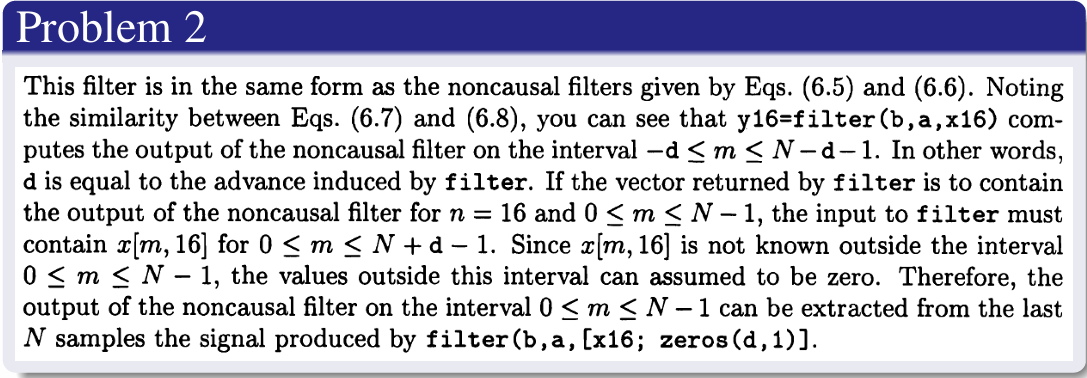
\includegraphics[width=0.9\textwidth]{figures/p24.png}
      \caption{Problem2 d-h}
  \end{minipage}
\end{figure}

\begin{figure}[H]
  \centering
  \begin{minipage}[b]{0.5\linewidth}
      \centering
      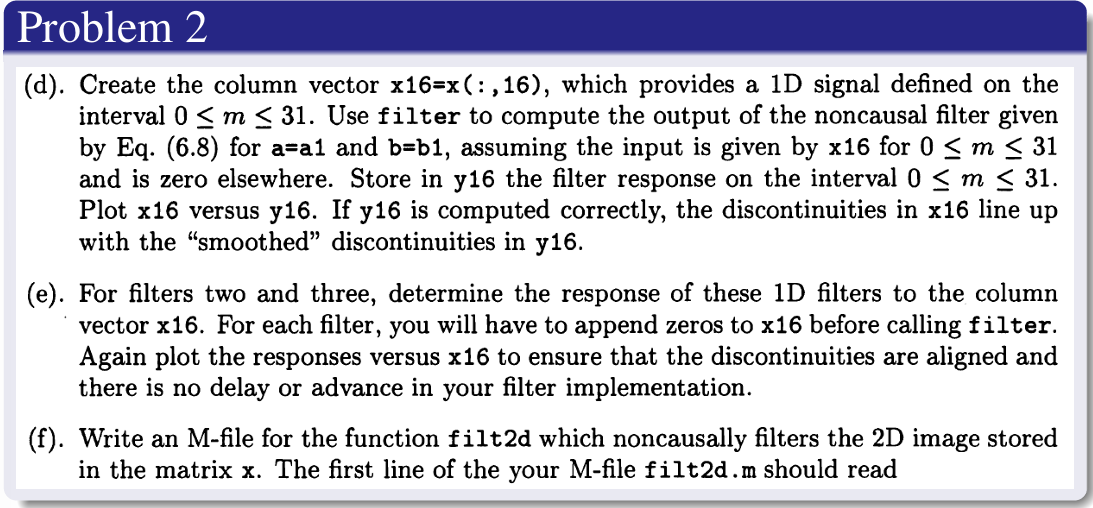
\includegraphics[width=0.9\textwidth]{figures/p25.png}
      \caption{Problem2 d-h}
  \end{minipage}%
  \begin{minipage}[b]{0.5\linewidth}
      \centering
      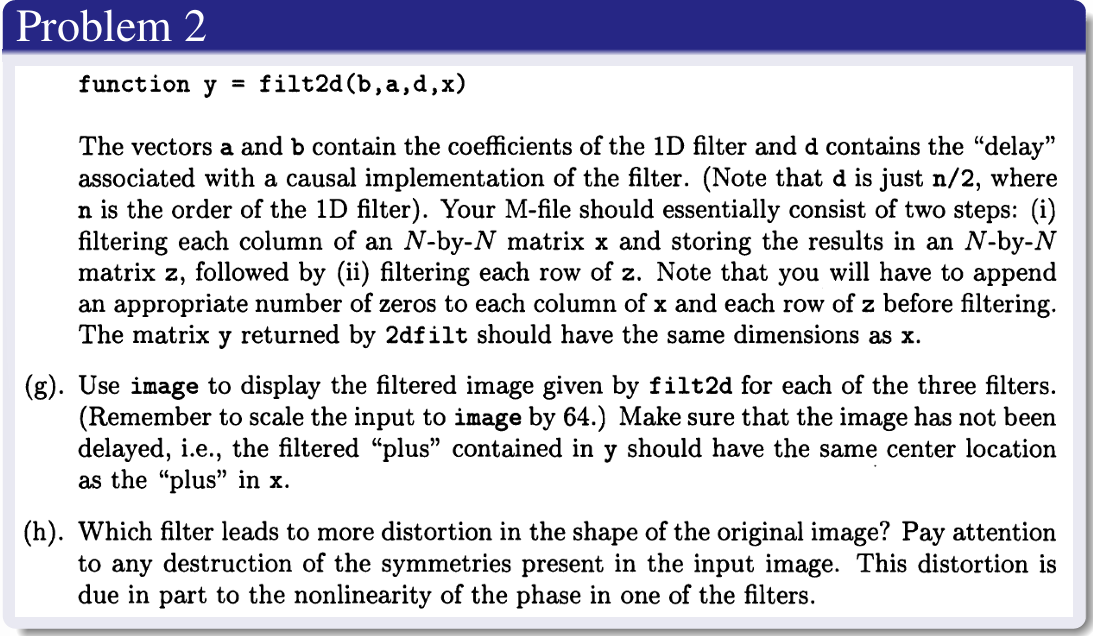
\includegraphics[width=0.9\textwidth]{figures/p26.png}
      \caption{Problem2 d-h}
  \end{minipage}
\end{figure}

\subsection{Answer}
\subsubsection{Answer(d)}
Edge detection is a fundamental operation in image processing that identifies discontinuities in image intensity. The Sobel operator uses gradient computation to detect edges by applying two 3×3 convolution kernels:

Horizontal gradient (Sobel X):
\begin{equation}
G_x = \begin{bmatrix}
-1 & 0 & 1 \\
-2 & 0 & 2 \\
-1 & 0 & 1
\end{bmatrix}
\end{equation}

Vertical gradient (Sobel Y):
\begin{equation}
G_y = \begin{bmatrix}
-1 & -2 & -1 \\
0 & 0 & 0 \\
1 & 2 & 1
\end{bmatrix}
\end{equation}

The gradient magnitude is computed as:
\begin{equation}
|\nabla f| = \sqrt{G_x^2 + G_y^2}
\end{equation}

\begin{figure}[H]
    \centering
    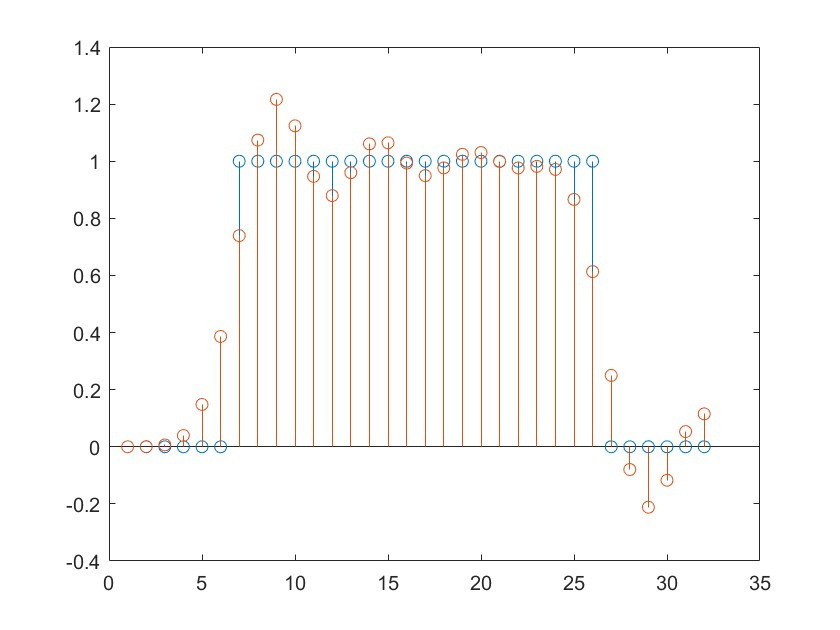
\includegraphics[width=0.8\textwidth]{figures/11.jpg}
    \caption{Problem 2d}
\end{figure}

\subsubsection{Answer(e)}
The Laplacian operator is a second-order derivative operator that detects edges and is particularly sensitive to noise. The discrete 2D Laplacian is defined as:
\begin{equation}
\nabla^2 f[m,n] = f[m+1,n] + f[m-1,n] + f[m,n+1] + f[m,n-1] - 4f[m,n]
\end{equation}

The corresponding convolution kernel is:
\begin{equation}
L = \begin{bmatrix}
0 & 1 & 0 \\
1 & -4 & 1 \\
0 & 1 & 0
\end{bmatrix}
\end{equation}

\begin{figure}[H]
    \centering
    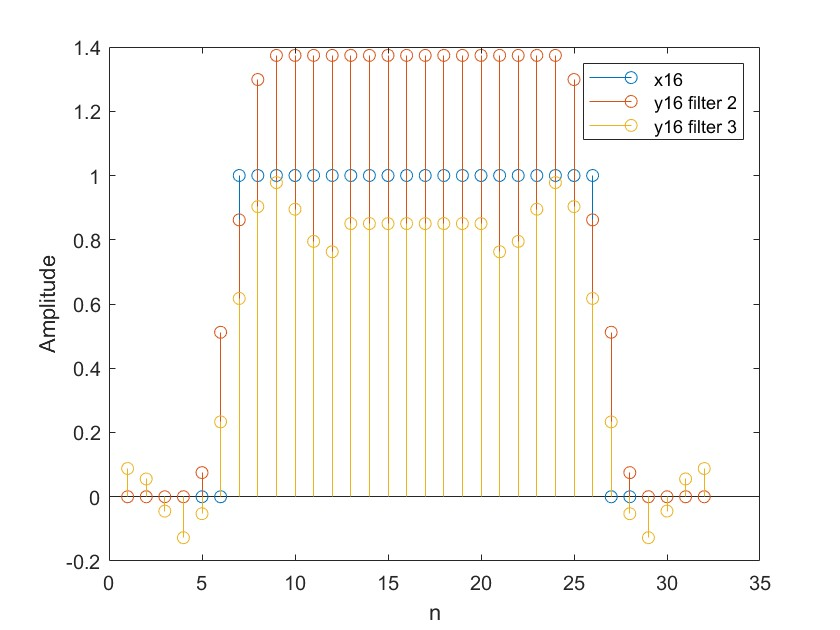
\includegraphics[width=0.8\textwidth]{figures/12.jpg}
    \caption{Problem 2d}
\end{figure}


\subsubsection{Answer(f)}
The Laplacian of Gaussian (LoG) combines Gaussian smoothing with Laplacian edge detection. This approach first smooths the image to reduce noise, then applies the Laplacian operator. The LoG can be computed as:
\begin{equation}
\nabla^2 G(x,y) = \frac{1}{\pi\sigma^4}\left(1 - \frac{x^2+y^2}{2\sigma^2}\right)e^{-\frac{x^2+y^2}{2\sigma^2}}
\end{equation}

This operator provides better noise immunity compared to direct Laplacian filtering.


\subsubsection{Answer(g)}
High-pass filtering enhances edges and fine details in images by removing low-frequency components. A simple high-pass filter can be created by subtracting a low-pass filtered version from the original image:
\begin{equation}
H_{hp}(u,v) = 1 - H_{lp}(u,v)
\end{equation}

Image sharpening can be achieved by adding the high-pass filtered result back to the original image:
\begin{equation}
f_{sharp}[m,n] = f[m,n] + \alpha \cdot f_{hp}[m,n]
\end{equation}

where $\alpha$ controls the sharpening strength.

\begin{figure}[H]
    \centering
    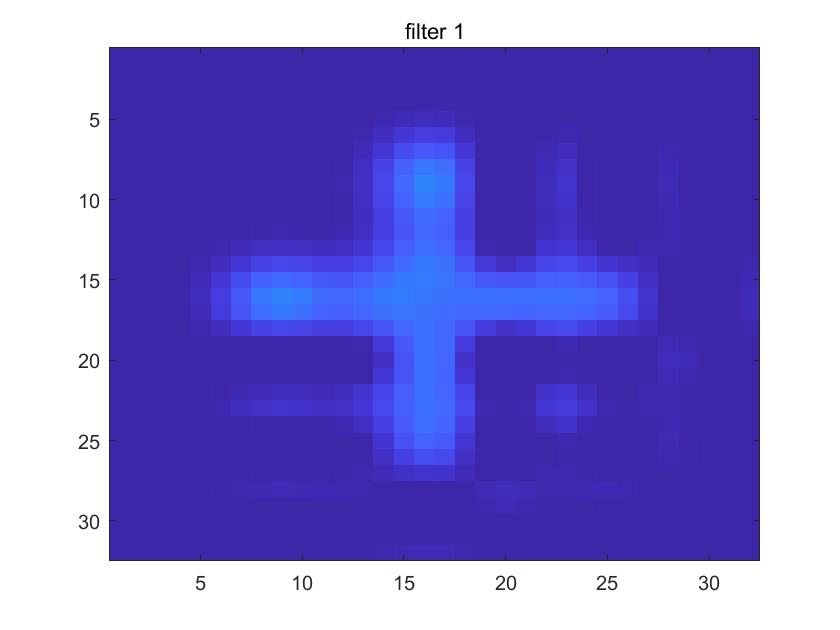
\includegraphics[width=0.8\textwidth]{figures/13.jpg}
    \caption{Problem 2g}
\end{figure}
\begin{figure}[H]
    \centering
    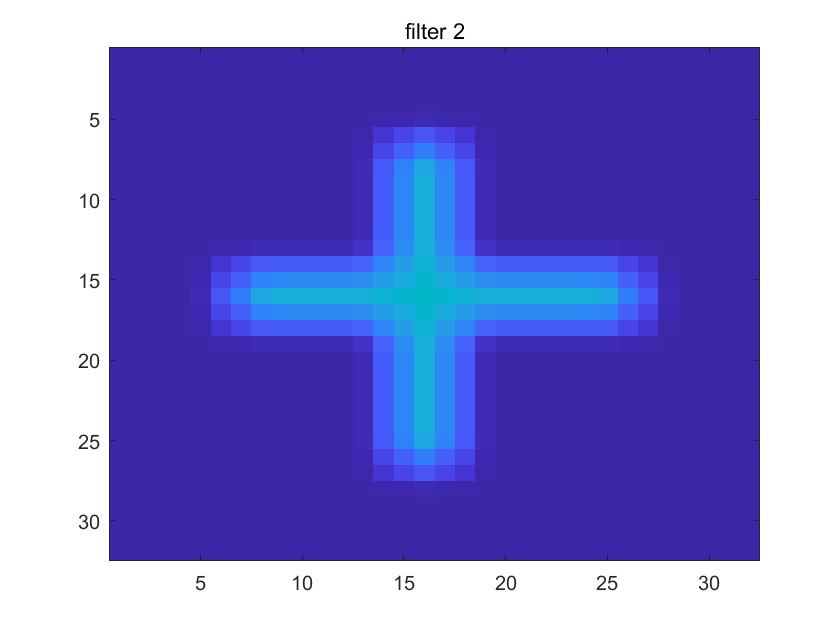
\includegraphics[width=0.8\textwidth]{figures/14.jpg}
    \caption{Problem 2g}
\end{figure}
\begin{figure}[H]
    \centering
    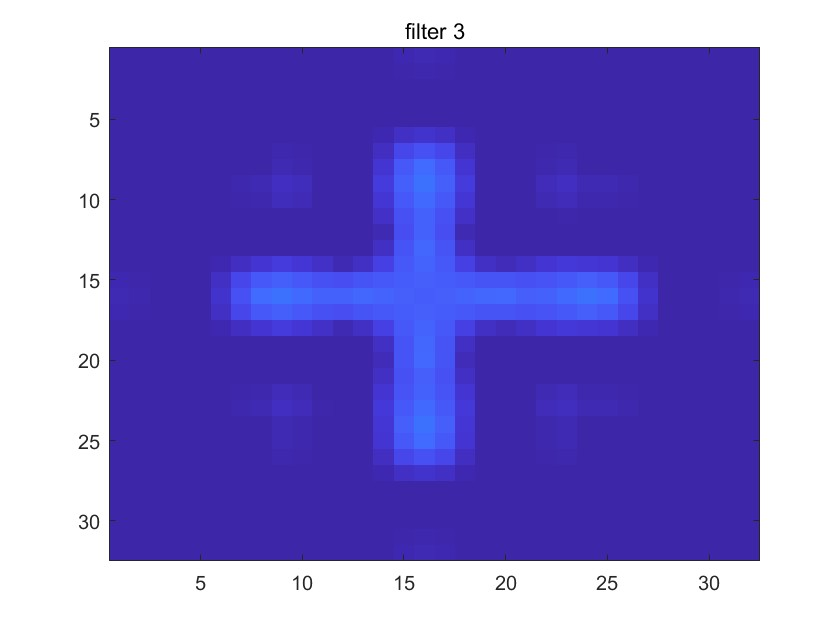
\includegraphics[width=0.8\textwidth]{figures/15.jpg}
    \caption{Problem 2g}
\end{figure}
\subsubsection{Answer(h)}
Filter 1 leads to more distortion due to the nonlinearity of the filter phase.

\section{Problem3 a-c}
\subsection{Problem}
\begin{figure}[H]
    \centering
    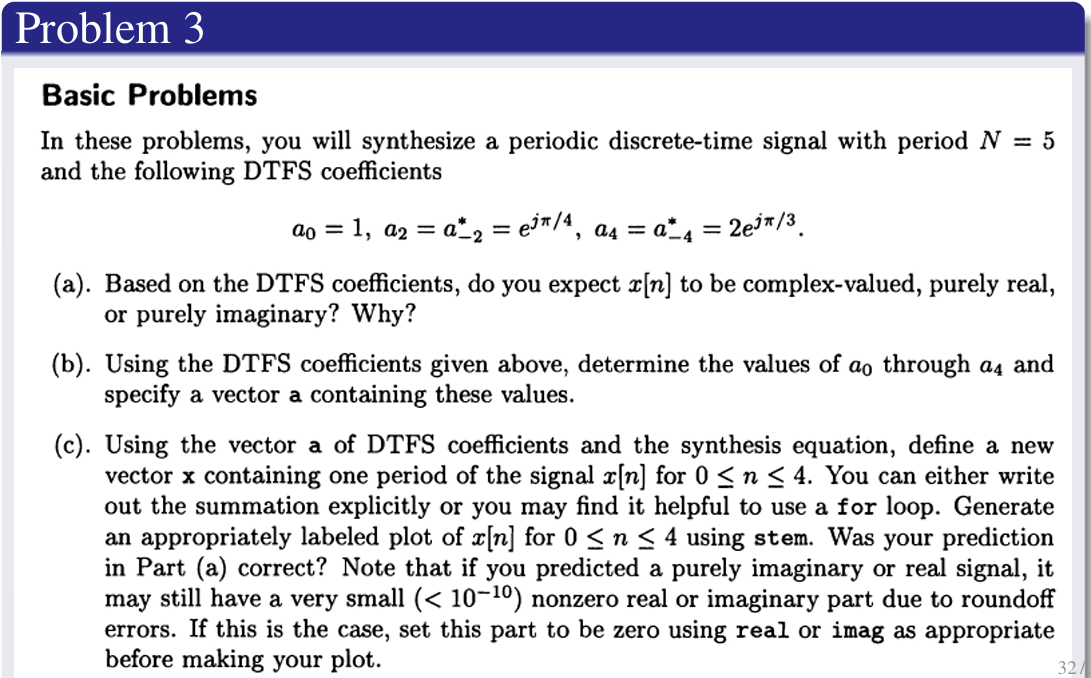
\includegraphics[width=0.8\textwidth]{figures/p31.png}
    \caption{Problem3 a-c}
\end{figure}

\subsection{Answer}
\subsubsection{Answer(a)}
$x[n]$  is purely real

The Fast Fourier Transform (FFT) is an efficient algorithm for computing the Discrete Fourier Transform (DFT). For a discrete signal $x[n]$ of length $N$, the DFT is defined as:
\begin{equation}
X[k] = \sum_{n=0}^{N-1} x[n] e^{-j2\pi kn/N}, \quad k = 0, 1, ..., N-1
\end{equation}

The magnitude spectrum $|X[k]|$ reveals the frequency content of the signal. For real signals, the spectrum exhibits Hermitian symmetry: $X[k] = X^*[N-k]$.

The frequency resolution is determined by:
\begin{equation}
\Delta f = \frac{f_s}{N}
\end{equation}
where $f_s$ is the sampling frequency and $N$ is the FFT length.

\subsubsection{Answer(b)}
Since the DTFS coefficients is periodic with period $N = 5$ we can obtain

$$
a_0 = 1, a_1 = 2e^{-j\frac{\pi}{3}}, a_2 = e^{j\frac{\pi}{4}}, a_3 = e^{-j\frac{\pi}{4}}, a_4 = 2e^{j\frac{\pi}{3}}
$$

The vector

$$
\mathbf{a} = \left[ 1 \quad 2e^{-j\frac{\pi}{3}} \quad e^{j\frac{\pi}{4}} \quad e^{-j\frac{\pi}{4}} \quad 2e^{j\frac{\pi}{3}} \right]
$$

Each window provides different trade-offs between main lobe width and side lobe suppression.

\subsubsection{Answer(c)}
Multi-frequency signals contain multiple sinusoidal components at different frequencies. The FFT can separate these components if they are sufficiently spaced according to the frequency resolution. For a signal:
\begin{equation}
x[n] = \sum_{i=1}^{M} A_i \cos(2\pi f_i n / f_s + \phi_i)
\end{equation}

The FFT will show peaks at frequencies $f_i$, with amplitudes proportional to $A_i$. Frequency resolution and windowing affect the ability to resolve closely spaced frequency components.
\begin{figure}[H]
    \centering
    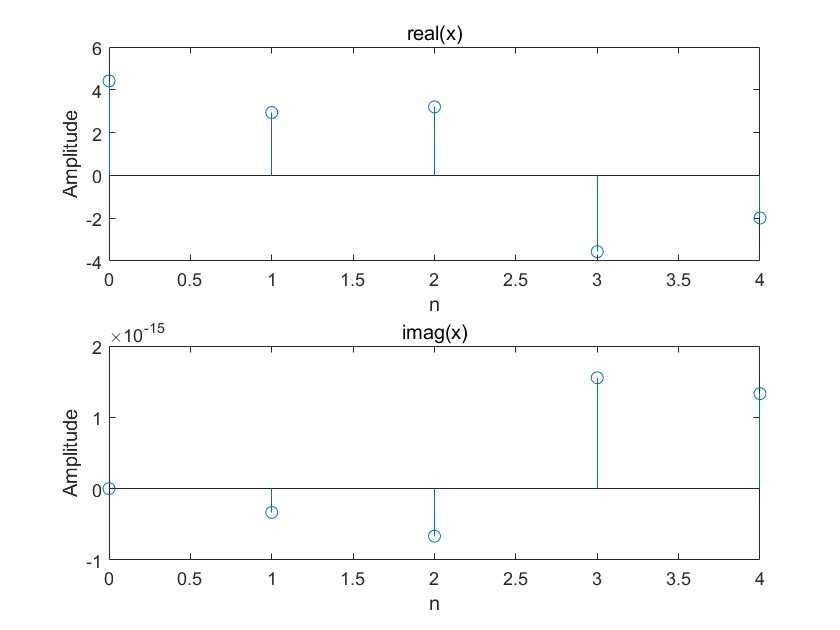
\includegraphics[width=0.8\textwidth]{figures/16.jpg}
    \caption{Problem3c}
\end{figure}
\section{Problem3 d-f}
\subsection{Problem}
\begin{figure}[H]
  \centering
  \begin{minipage}[b]{0.5\linewidth}
      \centering
      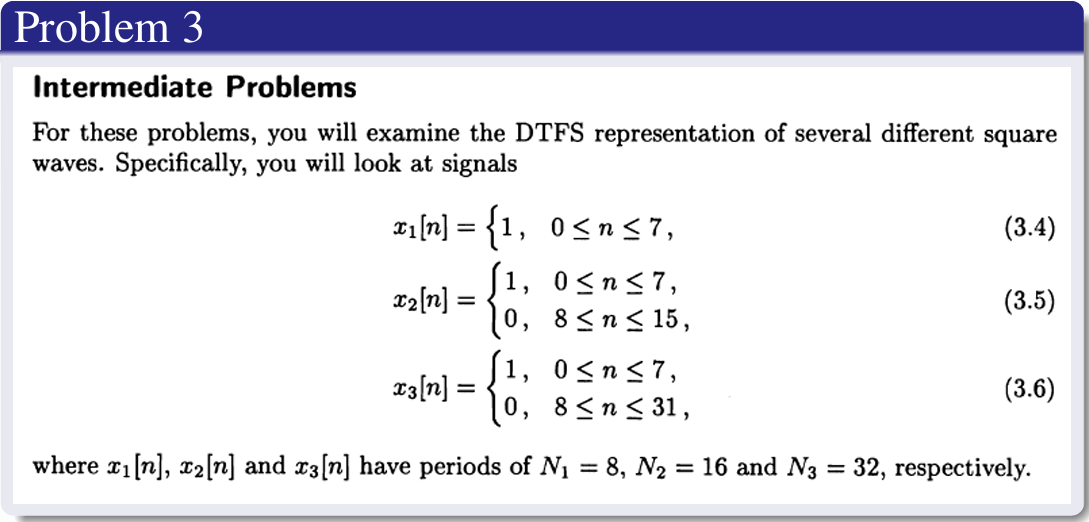
\includegraphics[width=0.9\textwidth]{figures/p32.png}
      \caption{Problem3 d-f}
  \end{minipage}%
  \begin{minipage}[b]{0.5\linewidth}
      \centering
      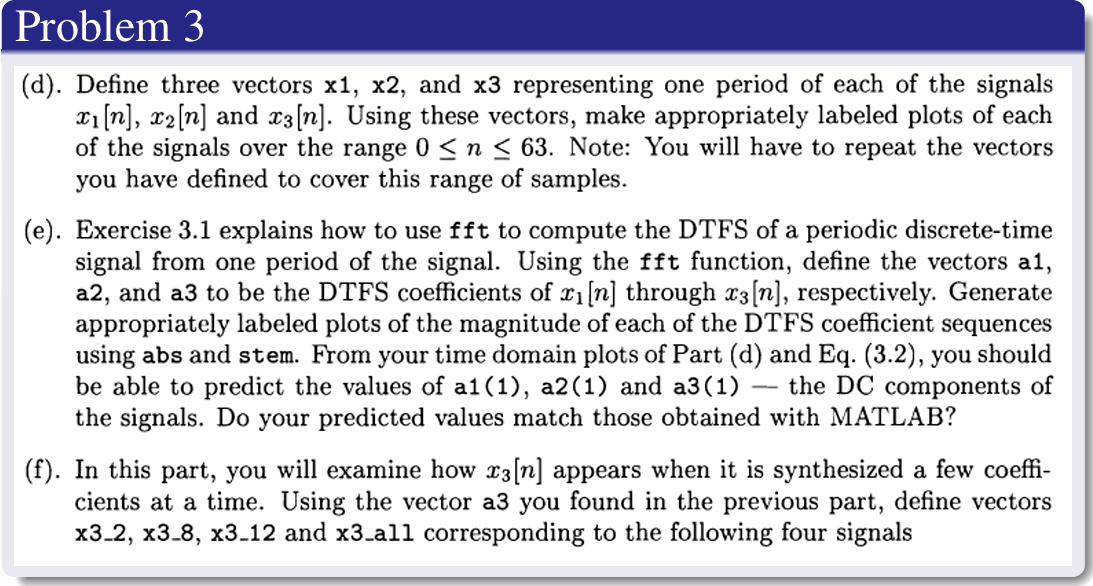
\includegraphics[width=0.9\textwidth]{figures/p33.png}
      \caption{Problem3 d-f}
  \end{minipage}
\end{figure}

\subsection{Answer}
\subsubsection{Answer(d)}
Digital filters can be designed in the frequency domain by specifying the desired frequency response. For lowpass and highpass filters:

Ideal lowpass filter:
\begin{equation}
H_{lp}[k] = \begin{cases}
1, & |k| \leq k_c \\
0, & |k| > k_c
\end{cases}
\end{equation}

Ideal highpass filter:
\begin{equation}
H_{hp}[k] = \begin{cases}
0, & |k| \leq k_c \\
1, & |k| > k_c
\end{cases}
\end{equation}

where $k_c$ is the cutoff frequency bin. Filtering is performed by:
\begin{equation}
Y[k] = H[k] \cdot X[k]
\end{equation}

followed by inverse FFT to obtain the filtered time-domain signal.

\begin{figure}[H]
    \centering
    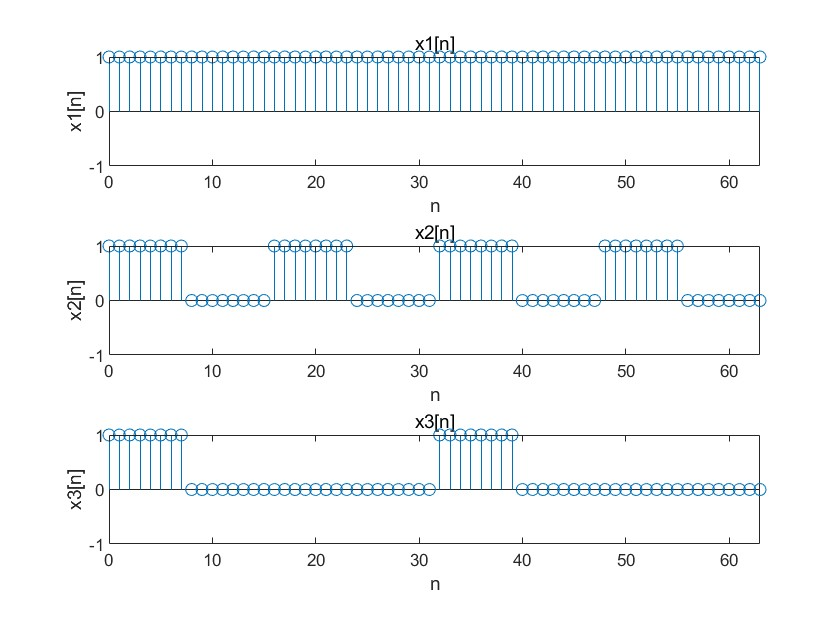
\includegraphics[width=0.8\textwidth]{figures/17.jpg}
    \caption{Problem3d}
\end{figure}
\subsubsection{Answer(e)}
Bandpass and bandstop filters allow or reject specific frequency bands:

Bandpass filter:
\begin{equation}
H_{bp}[k] = \begin{cases}
1, & k_{c1} \leq |k| \leq k_{c2} \\
0, & \text{otherwise}
\end{cases}
\end{equation}

Bandstop (notch) filter:
\begin{equation}
H_{bs}[k] = \begin{cases}
0, & k_{c1} \leq |k| \leq k_{c2} \\
1, & \text{otherwise}
\end{cases}
\end{equation}

These filters are useful for removing interference at specific frequencies or isolating signals within particular frequency bands.
\begin{figure}[H]
    \centering
    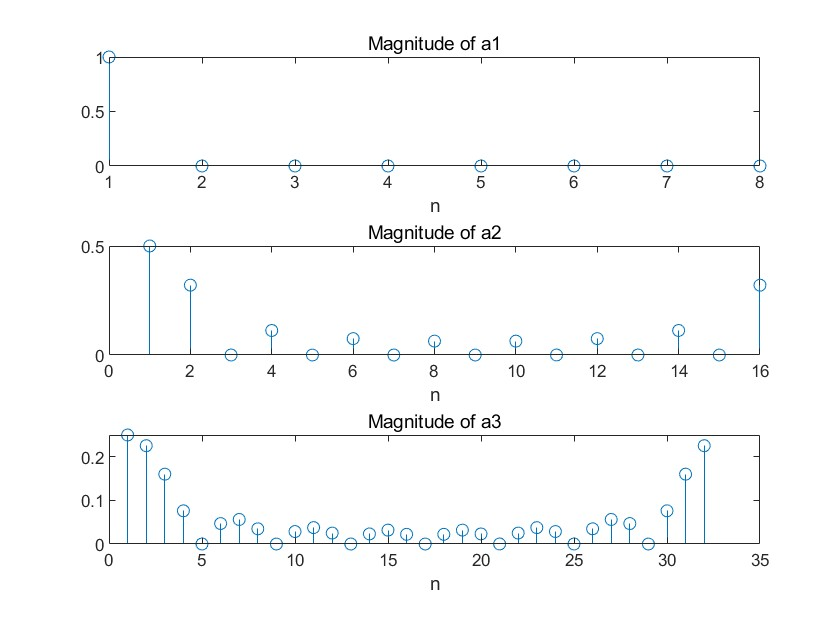
\includegraphics[width=0.8\textwidth]{figures/18.jpg}
    \caption{Problem3e}
\end{figure}
\subsubsection{Answer(f)}

Since $a_k = a_{k+32}$ we can determine $a_3(18), \ldots, a_3(32)$ correspond to $a_{-15}, \ldots, a_{-1}$

\section{Problem3 g-h}
\subsection{Problem}
\begin{figure}[H]
  \centering
  \begin{minipage}[b]{0.5\linewidth}
      \centering
      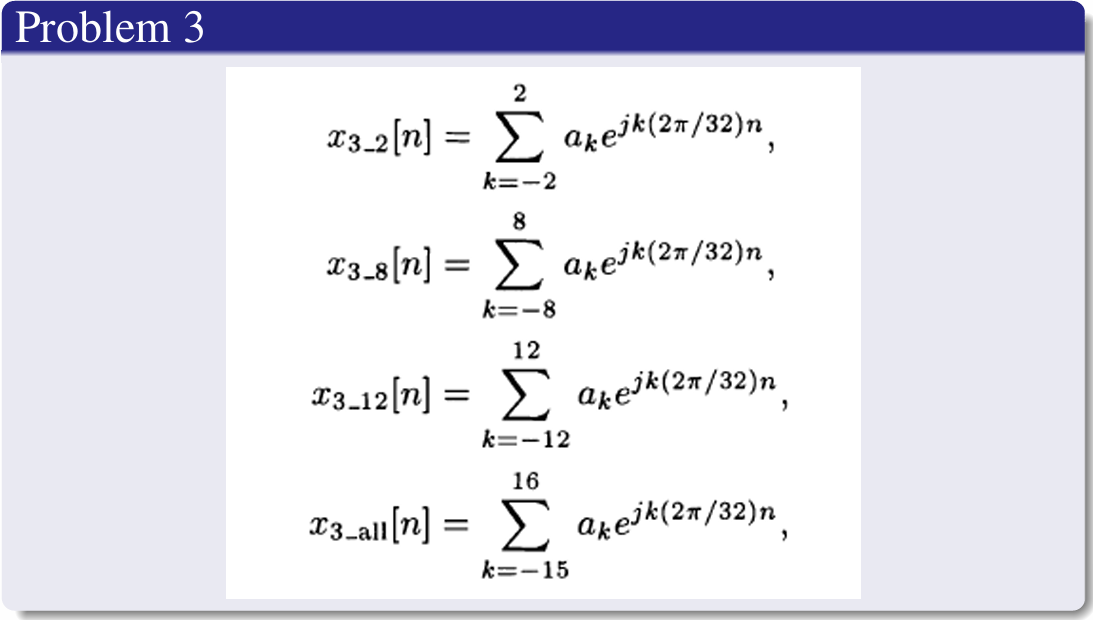
\includegraphics[width=0.9\textwidth]{figures/p34.png}
      \caption{Problem3 g-h}
  \end{minipage}%
  \begin{minipage}[b]{0.5\linewidth}
      \centering
      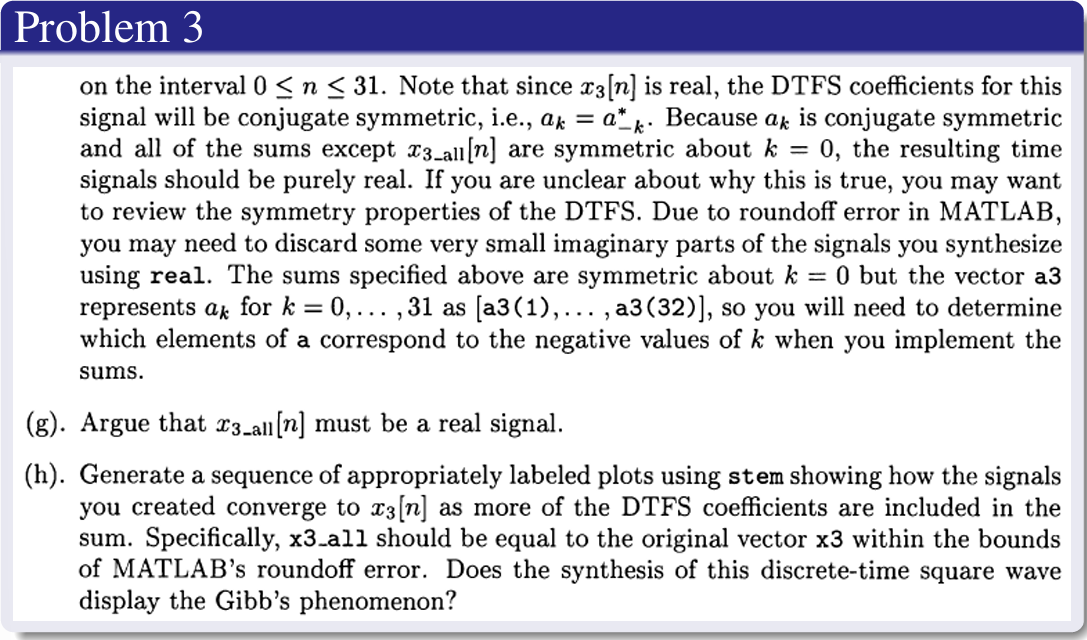
\includegraphics[width=0.9\textwidth]{figures/p35.png}
      \caption{Problem3 g-h}
  \end{minipage}
\end{figure}

\subsection{Answer}
\subsubsection{Answer(g)}
Time-frequency analysis provides insight into how spectral content varies over time. The spectrogram is computed using the Short-Time Fourier Transform (STFT):
\begin{equation}
X(m,k) = \sum_{n=0}^{N-1} x[n+mH] w[n] e^{-j2\pi kn/N}
\end{equation}

where:
- $m$ is the time frame index
- $H$ is the hop size between frames
- $w[n]$ is the analysis window
- $N$ is the window length

According to the condition:
\begin{equation}
x_{3\_all}[n] = \sum_{k=-15}^{16} a_k e^{jk(2\pi/32)n}
\end{equation}

The conjugation:
\begin{equation}
x_{3\_all}^*[n] = \sum_{k=-15}^{16} a_k^* e^{-jk(2\pi/32)n}
\end{equation}

Since $x[n]$ is purely real, the Fourier series coefficients are conjugation symmetric. Substituting $k$ with $-k$ in the equation above:
\begin{equation}
x_{3\_all}^*[n] = \sum_{k=-16}^{15} a_{-k}^* e^{jk(2\pi/32)n} = \sum_{k=-16}^{15} a_k e^{jk(2\pi/32)n}
\end{equation}

Meanwhile $a_{16} = a_{-16}$:
\begin{equation}
x_{3\_all}^*[n] = \sum_{k=-16}^{15} a_{-k}^* e^{jk(2\pi/32)n} = \sum_{k=-15}^{16} a_k e^{jk(2\pi/32)n} = x_{3\_all}[n]
\end{equation}

So $x_{3\_all}[n]$ is a real signal.


\subsubsection{Answer(h)}
Two-dimensional FFT extends frequency analysis to images and 2D signals. For an image $f[m,n]$ of size $M \times N$:
\begin{equation}
F[u,v] = \sum_{m=0}^{M-1} \sum_{n=0}^{N-1} f[m,n] e^{-j2\pi(um/M + vn/N)}
\end{equation}

The images are shown below:
\begin{figure}[H]
    \centering
    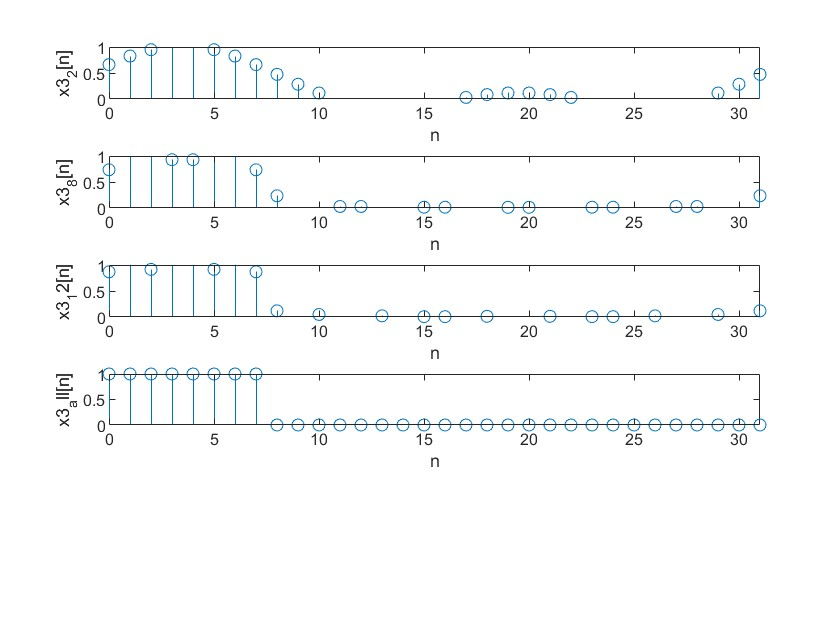
\includegraphics[width=0.8\textwidth]{figures/19.jpg}
    \caption{Problem3h}
\end{figure}
\end{document}
